En esta sección se describe técnicamente parte por parte cómo se ha planificado el proyecto.
El trabajo está dividido en tres secciones: análisis del código C, inyección de vulnerabilidades y soluciones a los retos.

En la primera sección, se explican las herramientas utilizadas para analizar los códigos fuentes de entrada y como se manejan los mismos.

La segunda sección, explica los diferentes tipos de vulnerabilidades que se pueden inyectar y como se modifica el código fuente original para poder incluir estos nuevos flujos y funciones vulnerables.

En la tercera y última sección, se explican los diferentes mecanismos de resolución del problema y cómo son entregados al usuario.
\section{Análisis del código fuente}
El proyecto está desarrollado en `Python', un lenguaje de programación sencillo que permite de forma rápida crear prototipos. En esta sección se describen las librerías, lógica y flujos que utiliza el programa.

\subsection{Preparación del entorno}
El desarrollo se ha realizado en un sistema operativo del tipo Linux, en concreto sobre la distribución de `Fedora', el software de este proyecto es compatible con cualquier sistema operativo de la familia Linux, que opere sobre arquitecturas del tipo \acrfull{x86} o \acrfull{x64}.

Más adelante se explican las diferencias que tienen en la traducción al código máquina. Este programa va a trabajar mayoritariamente con la arquitectura \acrshort{x86}.

Las dependencias del sistema necesarias para trabajar con el proyecto son las siguientes:
\begin{itemize}
    \item Sistema operativo
    \begin{itemize}
        \item \acrshort{gcc}
        \item glibc-devel.i686 (Paquete para compilar binarios de 32bit)
        \item glibc-devel.x86\_64
        \item python3.12
        \item poetry \cite{poetry-install}
        \item gdb
        \item gdb-server
        \item make
    \end{itemize}
    \item Librerías de Python para el proyecto
    \begin{itemize}
        \item pycparser \cite{pycparser}
        \item pwntools \cite{pwntools}
        \item structlog \cite{structlog}
    \end{itemize}
\end{itemize}

Las librerías de Python, se pueden instalar de forma automática mediante el gestor de paquetes `Poetry', para ello dentro del repositorio del proyecto, nos colocaremos en la carpeta `src' y podemos ejecutar dos comandos diferentes para conseguir el mismo objetivo, cualquiera de los dos instalará las dependencias necesarias a nivel de Python.

\begin{lstlisting}[language=bash]
# Usando el fichero Makefile
make init

# Comando manual de Poetry
poetry install
\end{lstlisting}

\subsection{Explicación del sistema AST}
El proyecto, hace uso de los \acrfull{ast} \cite{ast}. Un \acrshort{ast}, es una estructura de datos en forma de árbol que representa la estructura sintáctica abstracta de un texto escrito en un lenguaje formal, como código fuente. Cada nodo del árbol representa una construcción que ocurre en el texto. Los \acrshort{ast} son usados ampliamente en compiladores porque representan la estructura del código de un programa. La sintaxis abstracta se caracteriza por no incluir todos los detalles que se encuentran en la sintaxis concreta. Por ejemplo, la estructura de árbol subyacente implica el agrupamiento de los paréntesis, y una construcción sintáctica como IF condición THEN puede representarse con un único nodo que tenga dos ramas.

Esto es un ejemplo donde conviete el siguiente código Python sobre el algoritmo euclidiano a un \acrshort{ast}, mostrado en la figura \ref{fig:ast}:

\begin{lstlisting}[language=Python, caption=Python - Algoritmo euclidiano]
def euclidean(a: int, b: int) -> int:
    while b != 0:
      if a > b:
        a -= b
      else:
        b -= a
    return a
\end{lstlisting}

\begin{figure}[htb!]
      \centering                        
      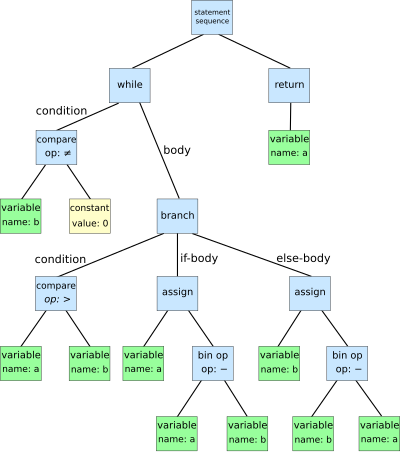
\includegraphics[width=0.8\textwidth]{images/AST.png}
      \caption{Algoritmo euclídeo en formato \acrshort{ast} }
      \label{fig:ast}
\end{figure}
\FloatBarrier
Como se puede observar en la figura \ref{fig:ast} este formato de árbol - rama no es sencillo de interpretar para un humano, sin embargo, de forma programática se puede analizar y/o alterar la estructura de forma relativamente sencilla.

El funcionamiento de la librería es complejo, por debajo emplea el metodo Lex (Lexer) - \acrfull{yacc}. Está implementado usando la librería `PLY' \cite{ply}, la cual es una herramienta que tokeniza el código y mediante funciones que analizan estos tokens permite construir un \acrshort{ast}, que es lo que realiza la herramienta `pycparser'.

\subsection{Análisis del código C con Python}
El software desarrollado implementa dos clases principales. La primera clase se encarga de procesar el código C, convertirlo en un \acrshort{ast} utilizando la librería `pycparser', y modificar este árbol para introducir cambios estructurales, como por ejemplo, las vulnerabilidades, esta clase se llama `AstProcessor'. La segunda clase se especializa en analizar el \acrshort{ast} generado, buscando puntos críticos donde se puedan inyectar vulnerabilidades de manera deliberada, tiene el nombre de `VulnGen'.

\subsubsection{AstProcessor}
Esta clase de Python únicamente hace uso de la librería `pycparser'. En ella se han implementado todas las funcionalidades importantes que permiten analizar, modificar, guardar y compilar el código.

El flujo para el procesado del código fuente comienza mediante el cargado del fichero en la librería. Para traducir el archivo a un \acrshort{ast}, el paquete hace uso de unas cabeceras modificadas de la \acrfull{libc} y del compilador \acrfull{gcc}. Para ello, las flags que se han añadido en el compilador son las siguientes:
\begin{itemize}
    \item -E : Afecta al enlazamiento de librerías
    \item -nostdinc : No incluir las librerías por defecto del sistema, por ejemplo, `string.h'
    \item -Iutils/fake\_libc\_include : Incluir las cabeceras falsas de libc para que el compilador no arroje errores
\end{itemize}

Una vez procesado el código al formato \acrshort{ast}, se hace un preprocesado de las secciones de interés para facilitar posteriores modificaciones y búsquedas de objetos. La clase dispone de 8 objetos principales diferentes:
\begin{itemize}
    \item ast: aquí se almacena todo el procesado obtenido por `pycparser'.
    \item astjson: lo mismo que en el objeto `ast', sin embargo, está en formato diccionario
    \item typedefs:  son definiciones de variables y tamaños sobre el nucleo de C.
    \item code: la subestructura del \acrshort{ast} con el código fuente importante, sin definiciones de tipos.
    \item funcs: diccionario con las definiciones de funciones
    \item globals: diccionario con variables globales o declaradas fuera de la función `main'
    \item vars: diccionario con todas las variables divididas en globales y funciones
    \item fncalls: diccionario con todas las llamadas a funciones divididas por función origen
\end{itemize}

Aprovechando el funcionamiento de las clases en Python, una modificación en cualquiera de los objetos enlazados entre variables repercutirá directamente sobre el objeto original debido a que el lenguaje referencia el valor original en vez de generar una nueva copia.

Para trabajar con el \acrshort{ast}, es muy importante entender el funcionamiento de los `scope' cuando se usa una variable en el código. El compilador primero intenta ubicar la variable en la función donde se está ejecutando, y en caso de no encontrar la variable, probará a buscarla de nuevo en el entorno global, siendo estrictos con la definición, un scope se define como código aislado entre dos llaves `\{\}'. Esto se puede comprobar con el siguiente código:
\pagebreak
\begin{lstlisting}[language=C, caption=Scopes en C]
int a = 1;
void b(){
    int a = 2;
    {
        int a = 3;
        printf("Subscope en la funcion b: %d\n", a);
    }
    printf("En la funcion b: %d\n", a);
}
int main()
{
    printf("En la funcion main: %d\n", a);
    b();
    return 0;
}
\end{lstlisting}

En el resultado se puede ver que arroja un texto con valor numérico diferente según el scope donde fue ejecutada la instrucción de imprimir por pantalla.

\subsubsection{VulnGen}
Esta clase de Python es la encargada de realizar un análisis del \acrshort{ast} e inyectar las vulnerabilidades propuestas en la sección \ref{subsec:vulns}. Es la clase más compleja del software debido a que tiene que ser capaz de encontrar funciones que permitan sustituirlas por sus análogas vulnerables, asegurando que la explotación sucede en el punto esperado.

La clase se construye sobre otras dos clases importantes: AstProcessor explicada en el punto anterior y la clase SAST, encargada de revisar el código y localizar posibles problemas.

\section{Vulnerabilidades}
\subsection{Buffer Overflow}
\subsection{Mitigaciones introducidas en el compilado}
\subsection{Evasión de mitigaciones}
\subsection{Inyección de vulnerabilidades} \label{subsec:vulns}
\section{Soluciones a los retos}
\subsection{Tutoriales}
\subsection{Ejemplos de Payloads}